\scanpage{20}\mspage{19}
% slanted
\margin{part of \deleted{\unsure{Theorem}} \unsure{theorem}}
\deleted{\uline{\unsure{Proposition}}}\inserted{\uline{Proposition} Let $X,Y$ be} Two closed tame subsets, in tame relative position. Then $X\cap Y$ is a \inserted{closed} tame subset, and
\[
\boxed{(X\cap Y)^{\cdot}\subset X^{\cdot}\cup Y^{\cdot}}
\]
Moreover, \inserted{$X$ and $Y$ have a supremum \unsure{in|in}} \deleted{among \unsure{all the} subsets} the set of tame subsets ordered by \deleted{closed tame which \unsure{contains} $X$} inclusion.
% slanted
\margin{\deleted{\unsure{Proof|Proof}} \uline{Proof} double induction on number of connected components of $X$ and of $Y$ (for the existence of the supremum and the question of boundaries)}
\deleted{$X$ and $Y$, and we} We write this subset $X\underset{\mathrm{mod}}{\cup}Y$, We have
\[
\boxed{(X\underset{\mathrm{mod}}{\cup}Y)^{\cdot}\subset X^{\cdot}\cup Y^{\cdot}}
\]
% slanted
\figure{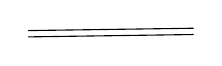
\begin{tikzpicture}[x=1cm,y=1cm]\draw (0,0)--(2.1,0.03);\draw (0,0.08)--(2.1,0.11);\end{tikzpicture}}
\margin{Remark, \unsure{every} tame subset $Z$ in \unsure{tame} relative position with $X$ and $Y$, is also so with $X\cap Y$ and $X\underset{\mathrm{mod}}{\cup}Y$}

\uline{Corollary} Let $(X_i)_{i\in I}$ be a finite family of closed tame subsets mutually in tame \deleted{relative} position. Then $\bigcap_i X_i$ is a tame subset, and the $X_i$ have a supremum in the set of closed tame subsets. We have
% slanted
\margin{\uline{Warning} for an \uline{arbitrary} subset $A$ of $\mathcal L$, there is in general \uline{no} closed tame closure, i.e. a ``smallest'' closed tame set $X$ such that $X\supset A$. This is already false in the standard case $L=[0,1]$ ! (Take $A=\{0,1/2,1/3\ldots\}$}
\[
\left(\bigcup_{\substack{\mathrm{mod}\\ i}} X_i\right)^{\cdot}\subset\bigcup_i X_i^{\cdot}
\]

\uline{Example}
\[
[a,b]\underset{\mathrm{mod}}{\cup}[b,c]=[a,c]
\]
but in general
\[
[a,b]\cup[b,c]\ne[a,c]
\]
(\unsure{take|when} $a$ least \unsure{c|e} element, $c$ greatest element \deleted{\unsure{and}} \unsure{arbitrary} \deleted{\unsure{And in this} $\unsure{=}$}, $b$ \deleted{\unsure{is}} comparable to every \inserted{element of $\mathcal L$.} If it is

% pale vertical watermark
% the paper's watermark (EXTRA STRONG), not his text
